%implementing document formatting:
\documentclass[a4paper,11pt,fleqn,dvipsnames,oneside,openright,oldfontcommands]{memoir} 	% Openright aabner kapitler paa hoejresider (openany begge)


%%%%%%%%% Indsat random
%makes it possible to refer to the name of a chapter rather than just the number.
\usepackage{nameref}
\usepackage{pdfpages}
\usepackage{marvosym}
\usepackage{setspace}
\usepackage{graphicx} % For at sætte 2 billeder ved siden af hinanden

%package for writing program code in latex
\usepackage{listings}
%%%%%%%%%%%%%%%%%%%%%%

% ¤¤ Oversaettelse og tegnsaetning ¤¤ %
\usepackage[T1]{fontenc}					% Output-indkodning af tegnsaet (T1)
\usepackage[danish]{babel}					% Dokumentets sprog
\usepackage[utf8]{inputenc}					% Input-indkodning af tegnsaet (UTF8)
\usepackage{ragged2e,anyfontsize}			% Justering af elementer
\usepackage{fixltx2e}						% Retter forskellige fejl i LaTeX-kernen							
				
																							
% ¤¤ Figurer og tabeller (floats) ¤¤ %
\usepackage{graphicx} 						% Haandtering af eksterne billeder (JPG, PNG, EPS, PDF)
%\usepackage{eso-pic}						% Tilfoej billedekommandoer paa hver side
%\usepackage{wrapfig}						% Indsaettelse af figurer omsvoebt af tekst. \begin{wrapfigure}{Placering}{Stoerrelse}
\usepackage{multirow}                		% Fletning af raekker og kolonner (\multicolumn og \multirow)
\usepackage{multicol}         	        	% Muliggoer output i spalter
\usepackage{rotating}						% Rotation af tekst med \begin{sideways}...\end{sideways}
\usepackage{colortbl} 						% Farver i tabeller (fx \columncolor og \rowcolor)
\usepackage{xcolor}							% Definer farver med \definecolor. Se mere: http://en.wikibooks.org/wiki/LaTeX/Colors
\usepackage{flafter}						% Soerger for at floats ikke optraeder i teksten foer deres reference
\let\newfloat\relax 						% Justering mellem float-pakken og memoir
\usepackage{float}							% Muliggoer eksakt placering af floats, f.eks. \begin{figure}[H]
\usepackage{array,booktabs,xcolor,longtable} % kan lave \hdashline i tabellertabe
\usepackage{arydshln}
\usepackage{tabu}

	
	
% ¤¤ Matematik mm. ¤¤
\usepackage{amsmath , amsthm , amsfonts , amssymb, float, stmaryrd} 		% Avancerede matematik-udvidelser
%\usepackage{mathtools}						% Andre matematik- og tegnudvidelser
\usepackage{textcomp}                 		% Symbol-udvidelser (f.eks. promille-tegn med \textperthousand )
\usepackage{rsphrase}						% Kemi-pakke til RS-saetninger, f.eks. \rsphrase{R1}
\usepackage[version=3]{mhchem} 				% Kemi-pakke til flot og let notation af formler, f.eks. \ce{Fe2O3}
\usepackage{siunitx}						% Flot og konsistent praesentation af tal og enheder med \si{enhed} og \SI{tal}{enhed}
\sisetup{output-decimal-marker = {,}}		% Opsaetning af \SI (DE for komma som decimalseparator) 

% ¤¤ Referencer og kilder ¤¤ %
\usepackage[danish]{varioref}				% Muliggoer bl.a. krydshenvisninger med sidetal (\vref)
\usepackage[numbers]{natbib}				% Udvidelse med naturvidenskabelige citationsmodeller
%\usepackage{xr}							% Referencer til eksternt dokument med \externaldocument{<NAVN>}
%\usepackage{glossaries}					% Terminologi- eller symbolliste (se mere i Daleifs Latex-bog)
\usepackage{lastpage}					% Gør det mulig at refere til sidste side 

% ¤¤ Misc. ¤¤ %
\usepackage{listings}						% Placer kildekode i dokumentet med \begin{lstlisting}...\end{lstlisting}
\usepackage{lipsum}							% Dummy text \lipsum[..]
\usepackage[shortlabels]{enumitem}			% Muliggoer enkelt konfiguration af lister
\usepackage{pdfpages}						% Goer det muligt at inkludere pdf-dokumenter med kommandoen \includepdf[pages={x-y}]{fil.pdf}	
\pdfoptionpdfminorversion=6					% Muliggoer inkludering af pdf dokumenter, af version 1.6 og hoejere
\pretolerance=2500 							% Justering af afstand mellem ord (hoejt tal, mindre orddeling og mere luft mellem ord)


% Kommentarer og rettelser med \fxnote. Med 'final' i stedet for 'draft' udloeser hver note en error i den faerdige rapport.
\usepackage[footnote,draft,danish,silent,nomargin]{fixme}		


%%%% CUSTOM SETTINGS %%%%

% ¤¤ Marginer ¤¤ %
\setlrmarginsandblock{3.0cm}{2.5cm}{*}		% \setlrmarginsandblock{Indbinding}{Kant}{Ratio}
\setulmarginsandblock{2.5cm}{3.0cm}{*}		% \setulmarginsandblock{Top}{Bund}{Ratio}
\checkandfixthelayout 						% Oversaetter vaerdier til brug for andre pakker

%	¤¤ Afsnitsformatering ¤¤ %
\setlength{\parindent}{6mm}           		% Stoerrelse af indryk
\setlength{\parskip}{0mm}          			% Afstand mellem afsnit ved brug af double Enter
\linespread{1,1}							% Linie afstand



% ¤¤ Indholdsfortegnelse ¤¤ %
\setsecnumdepth{subsection}		 			% Dybden af nummerede overkrifter (part/chapter/section/subsection)
\maxsecnumdepth{subsection}					% Dokumentklassens graense for nummereringsdybde
\settocdepth{subsection} 					% Dybden af indholdsfortegnelsen

% ¤¤ Lister ¤¤ %
\setlist{
  topsep=0pt,								% Vertikal afstand mellem tekst og listen
  itemsep=-1ex,								% Vertikal afstand mellem items
} 

%hyperlinks in the tabel of contents - comment this out before the report is printed.
\usepackage{hyperref}
\hypersetup{
	bookmarks = true,  % Show 'bookmark'-frame in pdf.
	colorlinks = true, % True = colored links, False = framed links.
	citecolor = black,  % Link color for references.
	linkcolor = black,  % Link color in table of contents.
	urlcolor = black,   % Link color for extern URLs.
}

% ¤¤ Opsaetning af figur- og tabeltekst ¤¤ %
\usepackage{caption}
%\usepackage{subcaption}
\captionnamefont{\small\bfseries\itshape}	% Opsaetning af tekstdelen ('Figur' eller 'Tabel')
\captiontitlefont{\small}					% Opsaetning af nummerering
\captiondelim{. }							% Seperator mellem nummerering og figurtekst
\hangcaption								% Venstrejusterer flere-liniers figurtekst under hinanden
%\captionwidth{0.9\textwidth}					% Bredden af figurteksten
\setlength{\belowcaptionskip}{0pt}			% Afstand under figurteksten
\captionsetup[figure]{labelfont={bf,it},font={it}} % sætter nummer til fed og kursis. Resten til fed + skriften er mindre end resten
\captionsetup[table]{labelfont={bf,it},font={it}} 


% ¤¤ Opsaetning af listings ¤¤ %

\definecolor{commentGreen}{RGB}{34,139,24}
\definecolor{stringPurple}{RGB}{208,76,239}

\lstset{language=Matlab,					% Sprog
	basicstyle=\ttfamily\scriptsize,		% Opsaetning af teksten
	keywords={for,if,while,else,elseif,		% Noegleord at fremhaeve
			  end,break,return,case,
			  switch,function},
	keywordstyle=\color{blue},				% Opsaetning af noegleord
	commentstyle=\color{commentGreen},		% Opsaetning af kommentarer
	stringstyle=\color{stringPurple},		% Opsaetning af strenge
	showstringspaces=false,					% Mellemrum i strenge enten vist eller blanke
	numbers=left, numberstyle=\tiny,		% Linjenumre
	extendedchars=true, 					% Tillader specielle karakterer
	columns=flexible,						% Kolonnejustering
	breaklines, breakatwhitespace=true,		% Bryd lange linjer
}

% ¤¤ Navngivning ¤¤ %
\addto\captionsdanish{
	\renewcommand\appendixname{Bilag}
	\renewcommand\contentsname{Indholdsfortegnelse}	
	\renewcommand\appendixpagename{Bilag}
	\renewcommand\appendixtocname{Bilag}
	\renewcommand\cftchaptername{\chaptername~}				% Skriver "Kapitel" foran kapitlerne i indholdsfortegnelsen
	\renewcommand\cftappendixname{\appendixname~}			% Skriver "Appendiks" foran appendiks i indholdsfortegnelsen
}

% ¤¤ Kapiteludssende ¤¤ %
%\definecolor{numbercolor}{gray}{0.7}		% Definerer en farve til brug til kapiteludseende
%\newif\ifchapternonum

\makechapterstyle{AAU}
{
	% Afstand mellem sidehovedet og kapitel+tal+kapitelnavnet defineres til:
	\setlength{\beforechapskip}{0cm}

	% Afstanden mellem kapitelnavnet og body-teksten defineres til:
	\setlength{\afterchapskip}{2cm}

	% Typografiopsætningen til kapitel+tal defineres til:
	\renewcommand\chapnamefont{\sffamily\bfseries\LARGE\raggedright}
	
	% Typografiopsætningen til kapitel+tal defineres til:
	\renewcommand\chaptitlefont{\sffamily\bfseries\huge\color[cmyk]{1.00,0.38,0.00,0.64}}

	% Forårsager, at der til kapitlet også tilføjes dets respektive tal:
	\renewcommand\chapternamenum{}
	\renewcommand\printchapternum
	{
		\makebox[0pt][l]
		{
			\color[cmyk]{1.00,0.38,0.00,0.64}
			\hspace{0.1cm}
			\resizebox{!}{1cm}{\chapnamefont\bfseries\sffamily\thechapter}
		}
	}
	
	% Definitionen af linjenstykket mellem ``Kapitel #'' samt ``kapitelnavnet'':
			\renewcommand\afterchaptertitle{\par\hspace{1.5cm}\hrule height 1pt\vskip\midchapskip}
}

% Aktivering af selve kapitellayoutet med dét navn, som definerer kapitellayoutet (ses fra tidligere):
\chapterstyle{AAU}

%\makechapterstyle{jenor}{					% Definerer kapiteludseende frem til ...
%  \renewcommand\beforechapskip{0pt}
%  \renewcommand\printchaptername{}
%  \renewcommand\printchapternum{}
% % \renewcommand\printchapternonum{\chapternonumtrue}
%  \renewcommand\chaptitlefont{\fontfamily{pbk}\fontseries{db}\fontshape{n}\fontsize{20}{25}\selectfont\raggedright}
%  \renewcommand\chapnumfont{\fontfamily{pbk}\fontseries{m}\fontshape{n}\fontsize{1in}{0in}\selectfont\color{numbercolor}}
% \renewcommand\printchaptertitle[1]{
%    \noindent
%    \ifchapternum
%     \begin{tabularx}{\textwidth}{XI}
%	{\let\\\newline\chaptitlefont ##1\par}     
%    \end{tabularx}
%    \par\vskip-2.5mm\hrule
%    \else
%    \begin{tabularx}{\textwidth}{X}
%      {\parbox[b]{\linewidth}{\chaptitlefont ##1}} & \raisebox{-15pt}{\chapnumfont \thechapter}
%    \end{tabularx}
%    \par\vskip2mm\hrule
%    \fi
%  }
%}											% ... her
%
%\chapterstyle{jenor}						% Valg af kapiteludseende - Google 'memoir chapter styles' for alternativer

% ¤¤ Sidehoved ¤¤ %

\makepagestyle{AAU}							% Definerer sidehoved og sidefod udseende frem til ...
\makepsmarks{AAU}{%
	\createmark{chapter}{left}{shownumber}{}{. \ }
	\createmark{section}{right}{shownumber}{}{. \ }
	\createplainmark{toc}{both}{\contentsname}
	\createplainmark{lof}{both}{\listfigurename}
	\createplainmark{lot}{both}{\listtablename}
	\createplainmark{bib}{both}{\bibname}
	\createplainmark{index}{both}{\indexname}
	\createplainmark{glossary}{both}{\glossaryname}
}
\nouppercaseheads											% Ingen Caps oenskes

\makeoddhead{AAU}{Gruppe 17gr6403}{}{\leftmark}				% Definerer lige siders sidehoved (\makeevenhead{Navn}{Venstre}{Center}{Hoejre})
\makeevenhead{AAU}{\rightmark}{}{Aalborg Universitet}		% Definerer ulige siders sidehoved (\makeoddhead{Navn}{Venstre}{Center}{Hoejre})
\makeevenfoot{AAU}{Side \thepage\ af \pageref{LastPage}}{}{}							% Definerer lige siders sidefod (\makeevenfoot{Navn}{Venstre}{Center}{Hoejre})
\makeoddfoot{AAU}{}{}{Side \thepage\ af \pageref{LastPage}}								% Definerer ulige siders sidefod (\makeoddfoot{Navn}{Venstre}{Center}{Hoejre})
\makeheadrule{AAU}{\textwidth}{0.5pt}						% Tilfoejer en streg under sidehovedets indhold
\makefootrule{AAU}{\textwidth}{0.5pt}{1mm}					% Tilfoejer en streg under sidefodens indhold

\copypagestyle{AAUchap}{AAU}								% Sidehoved for kapitelsider defineres som standardsider, men med blank sidehoved
\makeoddhead{AAUchap}{}{}{}
\makeevenhead{AAUchap}{}{}{}
\makeheadrule{AAUchap}{\textwidth}{0pt}
\aliaspagestyle{chapter}{AAUchap}							% Den ny style vaelges til at gaelde for chapters
															% ... her
															
\pagestyle{AAU}												% Valg af sidehoved og sidefod


%%%% CUSTOM COMMANDS %%%%

% ¤¤ Billede hack ¤¤ %
\newcommand{\figur}[4]{
		\begin{figure}[H] \centering
			\includegraphics[width=#1\textwidth]{billeder/#2}
			\caption{#3}\label{#4}
		\end{figure} 
}

% ¤¤ Specielle tegn ¤¤ %
\newcommand{\decC}{^{\circ}\text{C}}
\newcommand{\dec}{^{\circ}}
\newcommand{\m}{\cdot}


%%%% ORDDELING %%%%

\hyphenation{}

%%%%Fra engelsk til dansk i \autoref{•} %%%%
\renewcommand{\figureautorefname}{figur}
\renewcommand{\sectionautorefname}{afsnit}
\renewcommand{\subsectionautorefname}{afsnit}
\renewcommand{\subsubsectionautorefname}{afsnit}
\renewcommand{\tableautorefname}{tabel}
\renewcommand{\appendixautorefname}{bilag}
\renewcommand{\equationautorefname}{ligning}
\renewcommand{\itemautorefname}{punkt}
\renewcommand{\chapterautorefname}{kapitel}
%Figure references:
\newcommand{\figref}[1]{\textbf{figur \ref{#1}}}

%Figure references after full stop/period:
\newcommand{\Figref}[1]{\textbf{Figur \ref{#1}}}

%Table references:
\newcommand{\tableref}[1]{\textbf{tabel \ref{#1}}}

%Table references after full stop/period:
\newcommand{\Tableref}[1]{\textbf{Tabel \ref{#1}}}

%Units:
%inserting '\omit' before '{\put' prior ot final compile will fix allignment (and generate errors)
\newcommand{\unit}[1]{{\put(300,0){$\hfill\left[\: #1 \:\right]$}}}

%Text:
\newcommand{\tx}[1]{\text{#1}}

%Equation references:
%1 equation:
\renewcommand{\eqref}[1]{\textbf{ligning (\ref{#1})}}
%2 equations:
\newcommand{\eqrefTwo}[2]{\textbf{ligning (\ref{#1})} and \textbf{(\ref{#2})}}
%3 equations:
\newcommand{\eqrefThree}[3]{\textbf{ligning (\ref{#1})}, \textbf{(\ref{#2})} and \textbf{(\ref{#3})}}
%4 equations:
\newcommand{\eqrefFour}[4]{\textbf{ligning (\ref{#1})}, \textbf{(\ref{#2})}, \textbf{(\ref{#3})} and \textbf{(\ref{#4})}}
%5 equations:
\newcommand{\eqrefFive}[5]{\textbf{ligning (\ref{#1})}, \textbf{(\ref{#2})}, \textbf{(\ref{#3})}, \textbf{(\ref{#4})} and \textbf{(\ref{#5})}}
%5 equations:
\newcommand{\eqrefSix}[6]{\textbf{ligning (\ref{#1})}, \textbf{(\ref{#2})}, \textbf{(\ref{#3})}, \textbf{(\ref{#4})}, \textbf{(\ref{#5})} and \textbf{(\ref{#6})}}
%5 equations:
\newcommand{\eqrefSeven}[7]{\textbf{ligning (\ref{#1})}, \textbf{(\ref{#2})}, \textbf{(\ref{#3})}, \textbf{(\ref{#4})}, \textbf{(\ref{#5})}, \textbf{(\ref{#6})} and \textbf{(\ref{#7})}}

%Equation references after full stop/period:
%1 equation:
\newcommand{\Eqref}[1]{\textbf{Ligning (\ref{#1})}}
%2 equations:
\newcommand{\EqrefTwo}[2]{\textbf{Ligning (\ref{#1})} and \textbf{(\ref{#2})}}
%3 equations:
\newcommand{\EqrefThree}[3]{\textbf{Ligning (\ref{#1})}, \textbf{(\ref{#2})} and \textbf{(\ref{#3})}}
%4 equations:
\newcommand{\EqrefFour}[4]{\textbf{Ligning (\ref{#1})}, \textbf{(\ref{#2})}, \textbf{(\ref{#3})} and \textbf{(\ref{#4})}}
%5 equations:
\newcommand{\EqrefFive}[5]{\textbf{Ligning (\ref{#1})}, \textbf{(\ref{#2})}, \textbf{(\ref{#3})}, \textbf{(\ref{#4})} and \textbf{(\ref{#5})}}
%5 equations:
\newcommand{\EqrefSix}[6]{\textbf{Ligning (\ref{#1})}, \textbf{(\ref{#2})}, \textbf{(\ref{#3})}, \textbf{(\ref{#4})}, \textbf{(\ref{#5})} and \textbf{(\ref{#6})}}
%5 equations:
\newcommand{\EqrefSeven}[7]{\textbf{Ligning (\ref{#1})}, \textbf{(\ref{#2})}, \textbf{(\ref{#3})}, \textbf{(\ref{#4})}, \textbf{(\ref{#5})}, \textbf{(\ref{#6})} and \textbf{(\ref{#7})}}
\raggedbottom % Soerger for at LaTeX ikke "straekker" teksten

\begin{document}


\frontmatter	 % Forindhold - nummereres med romertal

%implementing title sheet:
\clearpage
\thispagestyle{empty}

%\begin{figure}[H]
%	\raggedleft
%		
\includegraphics[width=0.2\textwidth]{figures/aaulogo-da.png}
%\end{figure}


%\vspace*{\fill} 
%\begin{center}	
%	\begin{Huge}
%		P3 Projektrapport - efterår 2015\\
%		\vspace{5 mm}
%		\textbf{System til detektering af kropsbalance}\\
%		\vspace{3 mm}
%		Gruppe 375
%	\end{Huge}
%\end{center}
%\vspace*{\fill}

\begin{center}
\vspace*{\baselineskip}
\rule{\textwidth}{1.6pt}\vspace*{-\baselineskip}\vspace*{2pt} % Thick horizontal line
\rule{\textwidth}{0.4pt}\\[\baselineskip] % Thin horizontal line

{\huge Titel \\[0.4\baselineskip] \LARGE Projektrapport 6. semester}\\[0.2\baselineskip] % Title

\rule{\textwidth}{0.4pt}\vspace*{-\baselineskip}\vspace{3.2pt} % Thin horizontal line
\rule{\textwidth}{1.6pt}\\[\baselineskip] % Thick horizontal line
\vspace*{3\baselineskip}

%\scshape % Small caps
%Aalborg universitet,  01/02/16 - XX/XX/16\par % Location and year

%\vspace*{2\baselineskip} % Whitespace between location/year and editors

Skrevet af \\
{\Large Gruppe 17gr6XXX\par}
\end{center} % Center all text
{\color{white}X \\ X \\ X \\}
\begin{figure}[H]
	\centering
	\begin{minipage}[b]{1\textwidth}
		
\includegraphics[width=\textwidth]{figures/Forside}
	\end{minipage}
	\hfill
\end{figure}

\vspace*{\fill}
\begin{center}
	\textit{Gruppemedlemmer:}\\
	Birgithe Kleemann Rasmussen, Linette Helena Poulsen, Mads Kristensen \& Maria Kaalund Kroustrup \\
\end{center}
\begin{center}
\line(1,0){400}
\end{center}

%\begin{document} 
\thispagestyle{empty}
%\begin{titlepage}
\begin{nopagebreak}
	{\samepage 
		
		\begin{tabular}{r}
			\parbox{\textwidth}{  \raisebox{11mm}{
\includegraphics[height=2cm]{figures/aaulogo-da.png}}
				\hfill \hspace{2cm} \parbox{8cm}{\begin{tabular}{l} %4.90
						{\small \textbf{\textcolor{MidnightBlue}{{$6$. Semester}}}}\\
						{\small \textbf{\textcolor{MidnightBlue}{School of Medicine and Health}}}\\
						%{\small \textbf{\textcolor{MidnightBlue}{}}}\\ 
						{\small \textbf{\textcolor{MidnightBlue}{Sundhedsteknologi}}}\\
						{\small \textcolor{NavyBlue}{Fredrik Bajers Vej $7$A}} \\
						{\small \textcolor{NavyBlue}{$9220$ Aalborg}} \\
						%{\small \textcolor{NavyBlue}{\emph{http://www.smh.aau.dk/}}}
			\end{tabular}}}
		\end{tabular}
		
		\begin{tabular}{cc}
			\parbox{7cm}{
				\begin{description}

\item {Titel:} \\
Applikation til rehabilitering af  patienter med kronisk obstruktiv lungesygdom\\

\item {Tema:} \\
Design af sundhedsteknologiske systemer \\

\end{description}

\parbox{8cm}{

\begin{description}
\item {Projektperiode:}\\
   P$6$, Foråret $2017$\\
   
\item {Projektgruppe:}\\
  $17$gr$6403$\\
  
\item {Medvirkende:}\\
Birgithe Kleemann Rasmussen \\
Linette Helena Poulsen\\
Mads Kristensen \\
Maria Kaalund Kroustrup\\



\hspace{2cm}
\item {Vejleder:}\\
Hovedevejleder: Lars Pilegaard Thomsen  \\ 
\end{description}

}
\begin{description}
\item {Sider: }
\item {Bilag: }
\item {Afsluttet: $XX$/$05$/$2017$}
\end{description}
\vfill } &
\parbox{7cm}{
  \vspace{.15cm}
  \hfill 
  \begin{tabular}{l}
  {Synopsis:}\bigskip \\
  \fbox{
    \parbox{6.5cm}{\bigskip
     {\vfill{\small %Introduktion

     \bigskip}}
     }}
   \end{tabular}}
\end{tabular}} \vspace{1.3cm}
\raggedleft
\textit{\tiny Offentliggørelse af rapportens indhold, med kildeangivelse, må kun ske efter aftale med forfatterne.}\nopagebreak
\\
\end{nopagebreak}
%\end{titlepage}
%\end{document}
 %	\cleardoublepage
\clearpage

%%%% Indholdsfortegnelse (TOC) %%%%
\phantomsection													% Kunstigt afsnit, som hyperlinks kan 'holde fast i'
\pdfbookmark[0]{Indholdsfortegnelse}{indhold}					% Tildeler en klikbar bookmark til den endelige PDF
\tableofcontents*												% Indholdsfortegnelsen (kaldet ToC) 
%\clearpage
%\addtocontents{toc}{\protect\newpage}							% Fremtvinger sideskift i ToC hvis noedvendig (der hvor koden placeres)

\mainmatter

%Introduktion--------------------------------
\chapter{Indledning} 
Kronisk obstruktiv lungesygdom (KOL) er en kronisk inflammatorisk lungesygdom, der ødelægger bronkiernes vægge og/ellers danner forsnævringer i luftvejene. Dette forårsager, at lungefunktionen gradvist nedsættes.\cite{Basisbogen2016}

I Danmark er der ca. 430.000 mennesker med KOL, hvortil der er en årlig mortalitet på 3.500. Dette gør KOL til den fjerde hyppigste dødsårsag i Danmark.\cite{Basisbogen2016} På verdensplan er KOL på nuværende tidspunkt den tredje hyppigste dødsårsag \cite{WHO2017}.

KOL opstår som ofte af skadelige partikler samt gasser og miljøpåvirkninger. Den hyppigste årsag til KOL er tobaksrygning, der fremskynder tabet af lungefunktionen.\cite{Basisbogen2016,dsam2016,Martinez2016} Miljøpåvirkninger kan blandt andet være dårligt arbejdsmiljø, som eksempelvis arbejde med asbest, eller opvækst i dårligt miljø, hvilket kan påvirke barnets lunger til ikke at udvikle sig ordentligt. Miljøpåvirkninger kan derved resultere i en accelererende reduktion i lungefunktionen.\cite{Martinez2016}

Lungefunktionen nedsættes gradvist over mange år, hvilket gør, at KOL først kommer til udtryk sent i sygeforløbet. Dette kan resultere i, at patienter først opsøger sin læge, når deres lungefunktion er halveret.\cite{dsam2016} Symptomer forbundet med KOL opleves som åndenød samt hoste ved fysisk aktivitet, derudover er der en tendens til hyppig eksacerbationer. Eksacerbationer er akut forværring af patientens tilstand, hvilket kræver behandling.\cite{Basisbogen2016,dsam2016}
Derudover er der en række komorbiditeter, der kan være forårsaget af åndenød samt svage perifere muskler, som opleves ved KOL. Disse fremtræder som kardiovaskulære sygdomme, type-2 diabetes, osteoporose, lungecancer og muskelsvækkelse.\cite{dsam2016} Dertil har tobaksrygning samt dårlig livsstil betydning for udvikling af disse komorbiditeter \cite{McCarthy2015}. Foruden de nævnte komorbiditet, kan patienterne ligeledes opleve psykiske komorbiditet, såsom depression og angst, da patienterne ofte isolere sig på grund af generne ved KOL.\cite{dsam2016}

KOL kan ikke helbredes, og det er dertil ikke muligt at genvinde den tabte lungefunktion. Dog er det muligt at forhindre yderligere tab af lungefunktionen forårsaget af KOL samt lindre patienters symptomer.\cite{Basisbogen2016} Dette leder op til følgende initierende problemstilling.


\section{Initierende problemstilling}
\textit{Hvordan er nuværende diagnosticering og behandling af patienter med kronisk obstruktiv lungesygdom, og hvilke rehabiliteringsmuligheder kan tilbydes?}

%-----------------------Problemanalyse---------------------------
\chapter{Problemanalyse}
***     HER SKAL STÅ EN INDLEDEND TEKST ****

***     UDDYB PROBLEMET, HVOR DET PASSER IND  	****


\section{Kronisk obstruktiv lungesygdom}
Kronisk obstruktiv lungesygdom (KOL) er en kronisk inflammatorisk sygdom, der resulterer i gradvist nedsat lungefunktion. Inflammationen opstår i luftvejene og lungevævet, hvilket forårsager, at bronkiernes vægge ødelægges og/eller luftvejene forsnævres. KOL er beslægtet med to patologier, herunder kronisk bronkitis og emfysem. KOL-patienter oplever ofte begge patologier, men omfanget af disse varierer fra patient til patient.\cite{Basisbogen2016}

Kronisk bronkitis er luftvejsinflammation, hvor bronkierne i slimhinden er beskadiget, hvilket medfører en øget slimproduktion. Derudover er antallet af cilia mindsket, hvormed transport af slim og støvpartikler fra bronkierne til svælget begrænses, hvorfor der opstår bakterielle infektioner.\cite{Frausing2011,Britannica2016} KOL-patienter med overvejende kronisk bronkitis betegnes blue bloater. Disse patienter har ofte lungeinfektioner, cor pulmonale, hvilket betegner en trykbelastet og med tiden udvidet hypertrofisk samt dårlig fungerende højre ventrikel. Derudover oplever patienter ofte  type 2 respirationssvigt, hvor iltniveauet er lavt og indhold af kuldioxid højt. Den dårlige ilttilførsel til ekstremiteter, huden samt læber vil medvirke til, at huden bliver blålig, hvorfor disse patienter omtales blue bloater.\cite{Healthguidances2016}

Emfysem skyldes, at lungernes volumen er øget grundet beskadiget lungevæv, herunder destruktion af elastiske fibre og nedbrydning af væggene i de små lungeblærer. Dette medfører, at overfladen som lungerne har til rådighed ved luftudvekslingen mindskes, hvormed små bronkier kan klappe sammen og derved lukke under ventilation.\cite{Frausing2011a,Flaschen-Hansen2008} KOL-patienter med overvejende emfysem betegnes pink puffer. Disse patienter lider ofte af alvorlig afmagring eller vægttab med tydelige tegn på nedbrydning af muskelmasse og fedtvæv. Deres brystkasse er tøndeformet og de oplever type 1 respirationssvigt. Type 1 respirationssvigt betegner et lavt iltniveau og normalt indhold af kuldioxid. Disse patienter omtales pink puffer, da deres kroppe ved vejrtrækning pustes op og huden bliver rødlig.\cite{Healthguidances2016}

KOL bestemmes ved ratioen mellem forceret eksspiratorisk volumen (FEV1) og forceret vitalkapacitet (FVC). FEV1 måles ud fra, hvad der udåndes i det første sekund efter en maksimal indånding. FVC er lungevolumen målt i liter. Ved tilfælde af KOL er FEV1/FVC under 70 \% af den forventede lungekapacitet.\cite{Basisbogen2016}

Der er flere disponerende faktorer til KOL heriblandt skadelige partikler samt gasser, miljøpåvirkninger og genetiske faktorer. Den hyppigste årsag til KOL er tobaksrygning, som fremskynder tab af lungefunktionen.\cite{dsam2016,Basisbogen2016,Martinez2016} Foruden tobaksrygning kan miljøpåvirkninger have betydning for udviklingen af KOL. Opvækst i et dårligt miljø vil kunne påvirke barnets lunger til ikke at udvikle sig ordentligt, hvilket kan resultere i en lavere FEV1. Derudover vil et dårligt arbejdsmiljø, som f.eks. arbejde med asbest, kunne medvirke til en accelererende reduktion i FEV1, der ligeledes kan øge risikoen for KOL.\cite{Martinez2016} 
%Dette betyder, at en lav eller en accelererende reduktion af FEV1 vil mindske FEV1/FVC-ratioen.  

\subsection{Symptomer}
KOL udvikles over mange år, dog vil patienten ikke bemærke sygdommen førend lungefunktionen er markant nedsat. Dette betyder, at KOL og dens symptomer som regel først kommer til udtryk efter 50 års-alderen\cite{Lange2015}. Dette kan betyde, at patienter først opsøger en læge, når deres lungefunktion er halveret \cite{dsam2016}.

Symptomer på KOL er åndenød og hoste ved fysisk aktivitet, der kan være med ekspektoration, som hos de fleste KOL patienter er klart eller hvidt.\cite{Basisbogen2016} Derudover er der en tendens til hyppig eksacerbationer, hvilket er tilfælde, hvor KOL-patienters tilstand forværres akut og kræver behandling. 
Symptomerne herunder opleves som øget åndenød, hoste samt grønt eller gulligt ekspektoration og øget purulens. Denne tilstand skyldes ofte infektioner med bakterier, hvilket udgør ca. 50 \% af tilfældene. Derudover kan virale infektioner samt luftforurening resultere i, at KOL-patienter oplever eksacerbationer.\cite{Basisbogen2016, dsam2016} 

Der er en række komorbiditeter, som hyppigt ses hos KOL-patienter, som desuden kan have en negativ påvirkning på patienternes livskvalitet og prognose. Ved årskontroller bør patienten tjekkes for de hyppigste komormiditeter; kardiovaskulære sygdomme, type-2 diabetes, osteoporose, lungecancer, muskelsvækkelse samt angst og depression.
Nogle af komorbiditeterne kan skyldes, at åndenød har medført et nedsat fysisk aktivitetsniveau og dermed svage perifere muskler samt vægttab. Desuden har rygning og generelt dårlig livsstil ligeledes betydning for udviklingen af disse komorbiditeter. \cite{dsam2016, McCarthy2015}
Psykiske komorbiditeter, ofte i form af depression og angst, har en øget forekomst hos patienter med en FEV1 værdi på under 50 \% af den forventede værdi. Desuden kan angst og depression udløses ved diagnosen af KOL. Den øgede risiko for psykiske lidelser skyldes, at KOL kan medføre social isolation og tab af sociale relationer, skyldfølelse, usikkerhed med hensyn til fremtiden. \cite{dsam2016}


\subsection{Diagnose}
Ved mistanke om KOL undersøges lungefunktionen ved spirometriundersøgelser, hvor FEV1 og FVC måles. Patienten foretager en maksimal inspiration, hvorefter FEV1 er den volumen, som udåndes i det første sekund af en forceret eksspiration. Denne værdi giver information om hastigheden, hvormed lungerne tømmes. FVC er en indikator for lungevolumen. Som tidligere nævnt vil obstruktivt nedsat lungefunktion ses ved en FEV1/FVC-ratio på under 70 \% af den forventede værdi. Der udføres desuden en reversibilitetstest for at sikre, at patienten ikke lider af astma. Her gives patienten broncodilatorer, som hos astmapatienter vil forbedre spirometrimålingen, mens lungefunktionen for KOL-patienter forbliver uændret.\cite{Basisbogen2016, Sundhed2013} 

\begin{figure} [H]
\centering
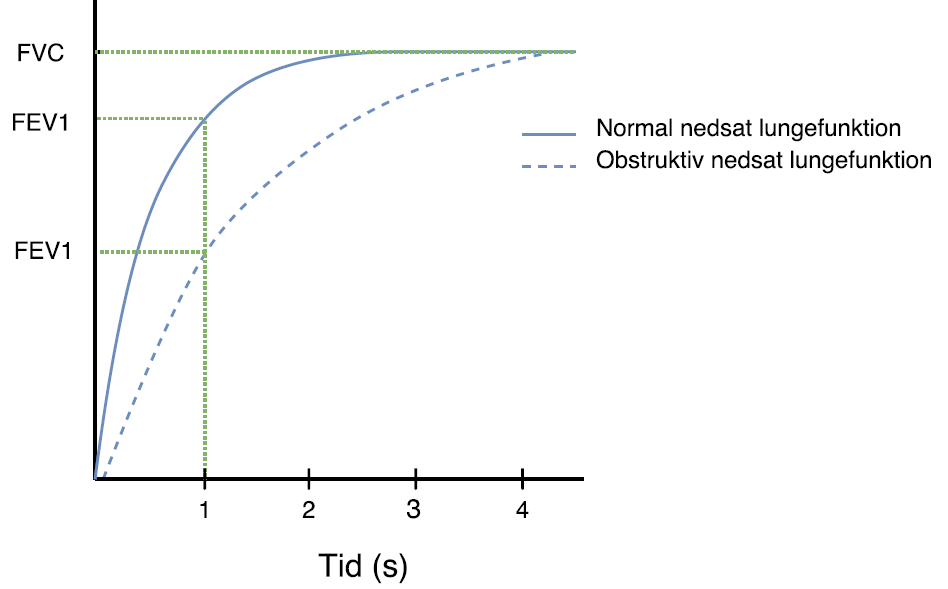
\includegraphics[width=0.5\textwidth]{figures/FEV}
\caption{Spirometrimåling ** MANGLER TEKST - MIDLERTIDIGT BILLEDE - DET SKAL TAGE UDGANGSPUNKT I BILLEDET FRA BASISBOGEN**}
\label{fig:FEV}
\end{figure} 

\noindent
** HER SKAL DER STÅ NOGET TEKST TIL BILLEDE ***

For at undersøge KOL og komobiditeter, som er forbundet med KOL undersøges foruden lungefunktionsundersøgelser BMI, røntgen af thorax, EKG-målinger og blodprøver \cite{Sundhed2013}. 
%Med tiden kan symptomerne på KOL forværres, og der skal mindre fysisk aktivitet til for at udløse åndenød. \cite{Basisbogen2016}
%%-----------------------System udvikling-------------------------



%%-----------------------Teori-------------------------




%%-----------------------Implementering-------------------------


%%-----------------------Test-------------------------%%


%\iffalse
\begingroup
\raggedright

\bibliographystyle{unsrtnat}
\bibliography{kilder123}
%\urlstyle{same}
%
%
%\printbibliography
%\cleardoublepage

\endgroup

%-----------------------Bilag-------------------------
\appendix
%\chapter{Bilag}
\chapter{Bilag}
\section{Lungernes anatomi og fysiologi} \label{BilagA}
Kroppens to lunger er omgivet af thorax og ligger i thoraxhulen. Thorax består af sternum og de ydre og indre interkostal muskler, herunder thorakal hvirvlerne, ribbenene samt musklerne mellem ribbenene. Halsmusklerne udgør loftet og diafragma udgør gulvet af sternum. De forskellige muskler og diafragma benyttes under ventilation. [1, 2]

\subsection{Ventilation}
Ventilation beskriver transport af luft frem og tilbage mellem atmosfæren og lungealveolerne. Luften bevæger sig fra områder med højt tryk til områder med lavt tryk. Det atmosfæriske tryk ændres ikke under normale omstændigheder, hvorfor det er variationer i trykket i alveolerne, der sørger for transporten af luft. Trykket skabes ved at lungerne udvides og presses sammen, herved bliver alveoletrykket lavere eller højere end det atmosfæriske tryk, hvilket medfører inspiration eller eksspiration. [1,2]

\subsubsection{Inspiration}
Inden inspiration er alle interkostal musklerne afslappede og alveoletrykket er det samme som det atmosfæriske tryk, hvilket betyder at der ikke strømmer luft gennem luftvejene. Ved inspiration udvides thoraxhulen, som medvirker til at trykket inde i lungen falder, hvormed  lungerne udvider sig. Kontraktion af interkostal musklerne øger volumen i både bredden og dybden. Diafragma trækker sig sammen medfører at thoraxhulens volumen øges. Halsmusklerne hæver ribbenene, hvilket yderligere medvirker til øget volumen af thoraxhulen. Når inspirationen er afsluttet afslappes interkostal musklerne igen. [1,2]

\subsubsection{Eksspiration}
Eksspiration sker når alveoletrykket inde i lungerne er større end det atmosfæriske tryk uden for. For at udligne trykket presses diafragma op mod sternum,interkostal musklerne trækker sig sammen, hvormed ribbene trækkes nedad. Dette medfører at lungernes volumen mindskes. Eksspirationen fortsættes indtil trykforskellen mellem det atmosfæriske tryk og alveoletrykket er udlignet. [1,2]

\subsection{Respiration}
Respirationssystemet består af et øvre og et nedre. Det øvre respirationssystem består af næsen, næsehulen, paranasal sinuses fxnote{er en gruppe af fire parrede luftfyldte rum, der omgiver næsehulen, herunder kæbehulerne, frontale bihuler, ethmoidale bihuler, sphenoidal bihuler.} og svælget. Det nedre respirationssystem indeholder larynx, trachea, bronkier, bronkioler og lungealveoler. [1,2]

\subsubsection{Transport af ilt} 
Ilten indtages i det øvre respirationssystem gennem næsen eller munden, herefter transporteres luften gennem trachea, hvor den deler sig i to hovedbronkier. Hovedbronkierne deler sig igen i mindre og mindre bronkier, hvor de til sidst ender i alveoler. Disse har udposninger yderst, kaldet bronkioler, og er omgivet af lungekapillærer.  Alveolevæggen er tynd, hvilket medvirker til at ilten kan diffundere over i blodet gennem lungekapillærer, hvorved blodet iltes og kan transporteres ud i musklerne. Modsat kan affaldsstoffet, kuldioxid, trænge fra blodet over i alveolerne, hvorved det kan udskilles ved eksspiration. [1,2]



%\fi
\end{document}
